\clearpage
\subsection{Procedure} % (fold)
\label{sub:procedure}

A Procedure is a part of a \nameref{sub:program} that performs a specific task. Each Procedure has a name that should reflect the task the procedure carries out. When a Procedure is called it gets control of the computer and instructs it to perform the steps needed to carry out the task the Procedure is responsible for. Often these tasks require data, so the Procedure may need to be passed data when it is called. When the procedure finishes its task control returns back to the code that called the Procedure.

\begin{figure}[h]
   \centering
   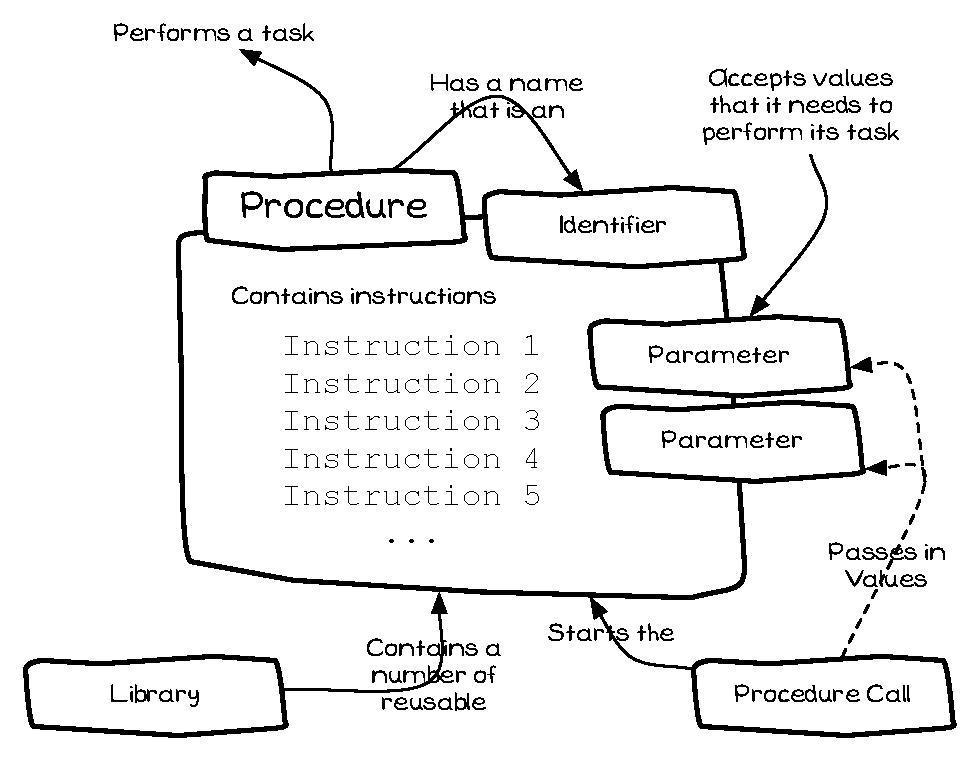
\includegraphics[width=\textwidth]{./topics/program-creation/diagrams/Procedure} 
   \caption[Procedure Concept Diagram]{A Procedure contains instructions to perform a task, and may need to be passed data in order to do this}
   \label{fig:program-creation-procedure}
\end{figure}


\mynote{
\begin{itemize}
  \item Figure \ref{fig:program-creation-procedure} shows the concepts related to Procedures.
  \item A Procedure is a programming artefact that can be called to perform a certain task.
  \item The name of a Procedure is an \nameref{sub:identifier}.
  \item Each \nameref{sec:program-creation-library} will contain a number of Procedures to perform common tasks.
  \item The standard library will include procedures to write values to the Terminal.
  \item The SwinGame libraries contain procedures that can draw images on the screen, play sounds, and perform other tasks needed to create small games.
  \item Procedures are also called \textbf{subroutines}, \textbf{sub programs}, \textbf{methods} or \textbf{sub procedures}.
\end{itemize}
}

% section program (end)